\documentclass{article}
\usepackage[utf8]{inputenc}
\usepackage{polski}

\usepackage{bbm}
\usepackage{graphicx}    
\usepackage{caption}
\usepackage{subcaption}
\usepackage{epstopdf}
\usepackage{amsmath,amssymb,amsfonts,amsthm,mathtools}
\usepackage{hyperref}
\usepackage{url}
\usepackage{alltt}
\usepackage{comment}
\usepackage[section]{placeins}
\graphicspath {{plots/}}
\newtheorem{defi}{Definicja}
\newtheorem{twr}{Twierdzenie}


\author{Jan Mazur 281141}
\date{Wrocław, \today}
\title{\textbf{Naturalne funkcje sklejane III stopnia} \\ Sprawozdanie do zadania P.2.9	}

\begin{document}
\maketitle

\section{Wstęp}

Interpolacja to proces polegający na wyznaczaniu w danym przedziale tzw. funkcji interpolacyjnej, która przyjmuje w nim z góry zadane wartości, w ustalonych punktach nazywanych węzłami. \cite{wikipedia_pl}
Często stosowana jest interpolacja wielomianowa, ponieważ  funkcje te mają sporo przydatnych własności, co implikuje istnienie wielu narzędzi matematycznych do ich analizy. Jednakże nie zawsze jest to dobra metoda.
Zastosować można wtedy inny sposób interpolacji - interpolację funkcjami sklejanymi.

Przedstawię obie metody, skupiając się jednak na interpolacji funkcjami sklejanymi. Porównam ich błędy w stosunku do funkcji interpolowanej.

Wszelkie testy i obliczenia zostały wykonane w środowisku Jupyter Notebook przy użyciu języka programowania \textbf{Julia} w wersji \textbf{0.5.0}.
Znaleźć można je w dołączonym do sprawozdania pliku \textbf{program.ipynb}.\\\\

\section{Interpolacja wielomianowa}
Interpolacja wielomianowa polega na znalezieniu wielomianu $n$-tego stopnia, który w $n+1$ węzłach będzie miał te same wartości co funkcja interpolowana. Rozważmy wielomiany interpolacyjne w postaci Newtona dla następujących funkcji:

\begin{equation}\label{fun1}
	f(x) = sin(x), \textnormal{ } x \in [0,\pi]
\end{equation}
\begin{equation}\label{fun2}
	f(x) = e^x, \textnormal{ } x \in [0,4]
\end{equation}
\begin{equation}\label{fun3}
	f(x) = (x^{2}+1)^{-1}, \textnormal{ } x \in [-5,5]
\end{equation}
\begin{equation}\label{fun4}
	f(x) = x/(x^{2} + \frac{1}{4}), \textnormal{ } x \in [-\pi,\pi]
\end{equation}

Przed przystąpieniem do obliczeń ustalmy najpierw funkcję błędu:
\begin{defi}\label{Error}
	$E_N^{(n)} := \max_{x \in D_N}|f(x)-s(x)))|$ \\
	\\
	Gdzie s jest funkcją interpolacyjną w n+1 parami różnych węzłach z przedziału $[a,b]$, f funkcją interpolowaną a $D_N$ zbiorem parami różnych równoodległych punktów z przedziału $[a,b]$.
\end{defi}

\renewcommand{\arraystretch}{1.5}  
\begin{center}
	\begin{tabular}{||c||c|c|c|c||} \hline
		\multicolumn{5}{||c||}{Tabela błędów dla N = 1000} \\ \hline
		Węzły 	& \multicolumn{4}{|c||}{Funkcje} \\ \cline{2-5}
				& $\sin x$ & $e^x$ & $(x^{2}+1)^{-1}$ & $x/(x^{2} + \frac{1}{4})$ \\ \hline					
		3 		& 5.59122e-02 &  1.80850e-03 &  2.90187e-07 & dupa\\\hline
		5 		& 5.60067e-02 &  1.80973e-03 &  2.99754e-07 & dupa\\\hline
		10  	& 5.60096e-02 &  1.81196e-03 &  3.00628e-07 & dupa\\\hline
		50  	& 5.60096e-02 &  1.81210e-03 &  3.00631e-07 & dupa\\\hline
		100  	& 5.60096e-02 &  1.81210e-03 &  3.00631e-07 & dupa\\\hline
	\end{tabular}

\end{center}
\renewcommand{\arraystretch}{1}

\begin{figure}[ht]
	\begin{center}
		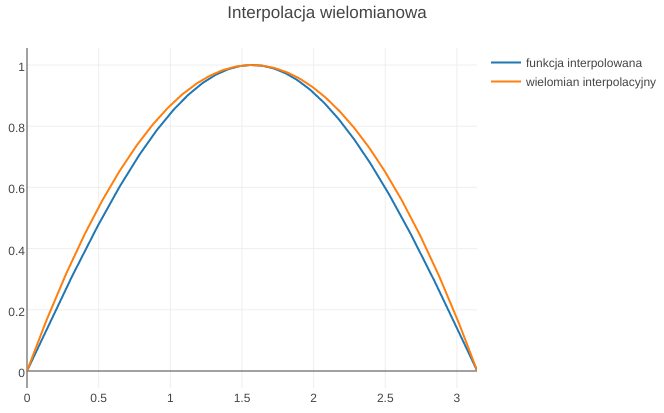
\includegraphics[width=13cm]{lagrange_sin}
	\end{center}
	\caption{Interpolacja funkcji \eqref{fun1} w 3 węzłach}
	\label{fig:rysunek1}
\end{figure}

\begin{figure}[ht]
	\centering
	\begin{subfigure}[ht]{0.5\textwidth}
		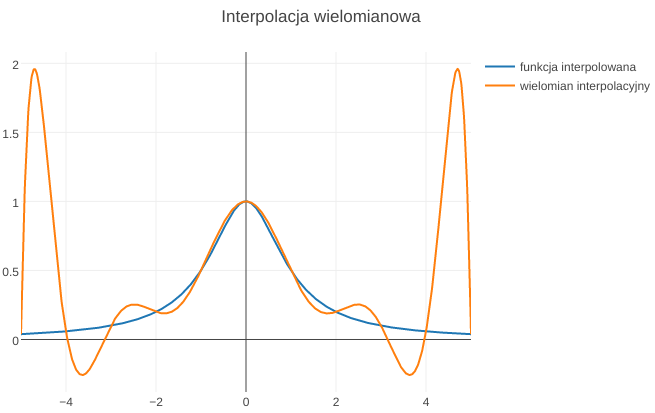
\includegraphics[width=\textwidth]{lagrange_c}
		\caption{Interpolacja funkcji \eqref{fun3}}
		\label{fig:2}
	\end{subfigure}%
	\begin{subfigure}[ht]{0.5\textwidth}
		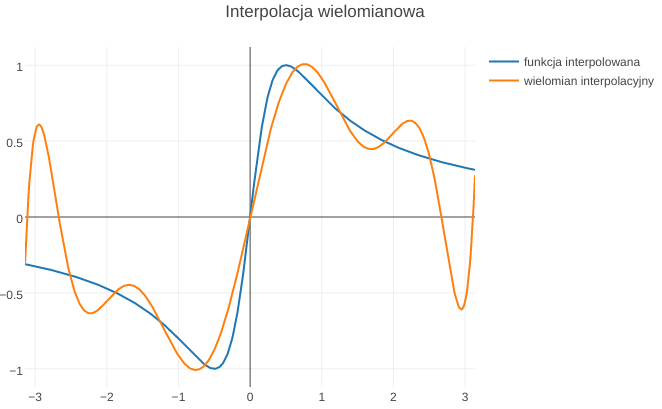
\includegraphics[width=\textwidth]{lagrange_d}
		\caption{Interpolacja funkcji \eqref{fun4}}
		\label{fig:3}
	\end{subfigure}
\end{figure}

W przypadku funkcji \eqref{fun1} i \eqref{fun2} błąd wielomianu interpolacyjnego jest niewielki. Natomiast przy funkcjach \eqref{fun3} i \eqref{fun4} zaobserwować można tzw. efekt Runge'go\cite{runge}. Polega on na tym, że przy zwiększaniu ilości węzłów uzyskujemy coraz większy błąd na końcach przedziałów interpolacji. Rozwiązaniem tego problemu może być interpolacja funkcjami sklejanymi.

Obliczenia dla innych funkcji i kombinacji punktów interpolacji oraz $N$ można znaleźć w pliku \textbf{program.ipynb}.

\section{Funkcje sklejane}


\begin{defi}
	\textbf{Funkcją sklejaną} S(x) stopnia s, określoną na przedziale $[a,b]$ nazywamy dowolną funkcję spełniającą warunki:
	
	\begin{itemize}
		\item w każdym przedziale $[t_i,t_{i+1}]$, gdzie $a = t_0 < t_i <...<t_n = b$, S jest wielomianem stopnia co najwyżej s.
		\item S oraz jej pochodne rzędu 1,2,...,s-1 są ciągłe na całym przedziale $[a,b]$.
	\end{itemize}
\end{defi}

\noindent Aby ujednoznacznić istnienie takiej funkcji n-tego stopnia wyznaczanej przez $n+1$ punktów $t_i$ definiuje się dodatkowe warunki:

\begin{defi}
	Funkcję sklejaną S(x) stopnia s, określoną na przedziale $[a,b]$
	nazywamy \textbf{naturalną} gdy:
	$S^{(s-1)}(a) = S^{(s-1)}(b) = 0$.
\end{defi}

Rozważmy interpolacje naturalną funkcją sklejaną III stopnia gdzie $t_i$ będą węzłami interpolacji.

\section{Interpolacja naturalną funkcją sklejaną III stopnia}

\begin{defi}
	Naturalna funkcja sklejana III stopnia S, interpolująca funkcję f w punktach $a = x_0 < x_i <...<x_n = b$ w przedziale $[a,b]$ spełnia warunki:
	
	\begin{itemize}
		\item w każdym przedziale $[x_i,x_{i+1}]$ S jest wielomianem stopnia co najwyżej 3.
		\item Dla wszystkich $x_i$ $S(x_i) = f(x_i)$.
	\end{itemize}
	
\end{defi}

\noindent Wprowadźmy oznaczenie:

\begin{defi}
	$M_k := S''(x_k)$
\end{defi}

\begin{twr}
	Wielkośći $M_k$ spełniają układ równań liniowych:\\
	$\lambda_k M_{k-1} + 2M_k + (1-\lambda_k) M_{k+1} = 6f[x_{k-1},x_k,x_{k+1}]$ \hfill $(k=0,1,...,n)$\\
	gdzie: $\lambda_k := h_k / ( h_k + h_{k+1})$, oraz $h_k = x_k - x_{k-1}$
\end{twr}
	
Układ równań z powyższego twierdzenia w postaci macierzowej ma trójprzekątniową macierz z dominującą przekątną. Można go więc rozwiązać w czasie liniowym.

\subsection{Algorytm rozwiązujący układ równań ze względu na $M_k$ w czasie linowym}

\begin{align}
	&q_0 := u_0 := 0 \\
	\notag
	&\begin{rcases}
		p_k := \lambda_k q_{k-1} + 2 \\ \notag
		q_k := (\lambda_k - 1) / p_k \\ \notag
		u_k := (d_k -\lambda_k u_{k-1}) / p_k
	\end{rcases}
	\text{$(k=1,2,...,n-1)$}
\end{align}
gdzie
\begin{equation*}
	d_k = 6 f[x_{k-1},x_k,x{k+1}] \textnormal{ } (k=1,2,...,n-1)
\end{equation*}
Wówczas
\begin{align*}
	&M_{n-1} = u_{n-1} \\ \notag
	&M_k = u_k + q_k M_{k+1} \textnormal{ } (k =n-2,n-3,...,1 )
\end{align*}
\\

\noindent Naturalna funkcja sklejana III stopnia interpolująca funkcję f w przedziale $[a,b]$ i punktach $a = x_0 < x_i <...<x_n = b$ dana jest wzorem:

\begin{align}
	S(x) = h_{k}^{-1}&[\frac{1}{6} M_{k-1}(x_k - x)^3  
					 +\frac{1}{6} M_k (x - x_{k-1})^3 \\
					 \notag
					 &+(f(x_{k-1}) - \frac{1}{6} M_{k-1} h_{k}^2) (x_k -x ) \\
					 \notag
					 &+(f(x_{k}) - \frac{1}{6} M_{k} h_{k}^2) (x_{k-1} -x )]
\end{align}


\section{Testy}
Po zaimplementowaniu algorytmu znajdującego naturalną funkcję sklejaną III stopnia dla danej funkcji interpolowanej wykonałem testy dla funkcji\eqref{fun1} \eqref{fun2} \eqref{fun3} \eqref{fun4}.
	
	
\section{Wnioski}
Jeśli zwykła interpolacja bardzo odstaje w niektórych miejscach to lepiej interpolować splinem.
Spliney dobrze odwzorowują kształt a niekoniecznie dokładne wartości funkcji.

Czy punkty równoodległe?


\begin{thebibliography}{9}
	\itemsep2pt
			
	\bibitem{kincaid} David Kincaid, Ward Cheney - "Analiza Numeryczna"
	
	\bibitem{prezentacja} \url{https://www.math.ntnu.no/emner/TMA4215/2008h/cubicsplines.pdf}
	
	\bibitem{wolfram_mathworld} Weisstein, Eric W. "Cubic Spline." From MathWorld--A Wolfram Web Resource. \url{http://mathworld.wolfram.com/CubicSpline.html}
	
	\bibitem{wiki} \url{https://en.wikipedia.org/wiki/Spline_interpolation}
	
	\bibitem{wikipedia_pl}
	\url{https://pl.wikipedia.org/wiki/Interpolacja_(matematyka)}
	
	\bibitem{runge}
	\url{https://en.wikipedia.org/wiki/Runge%27s_phenomenon}
	 
\end{thebibliography}

\end{document}